% Appendix B

\renewcommand{\appendixname}{Anexo}
\chapter{Ataque físico placas matrículas} % Main appendix title

\label{AppendixB} % For referencing this appendix elsewhere, use \ref{AppendixA}
\section{Placa matrícula alemana}
Ejemplos adversarios físicos de ataque de fuerza bruta para confundir la interpretación del dígito 1 en modelo Wpod-Net [60] con placa matrícula alemana.

\begin{figure}[!h]
    \centering
    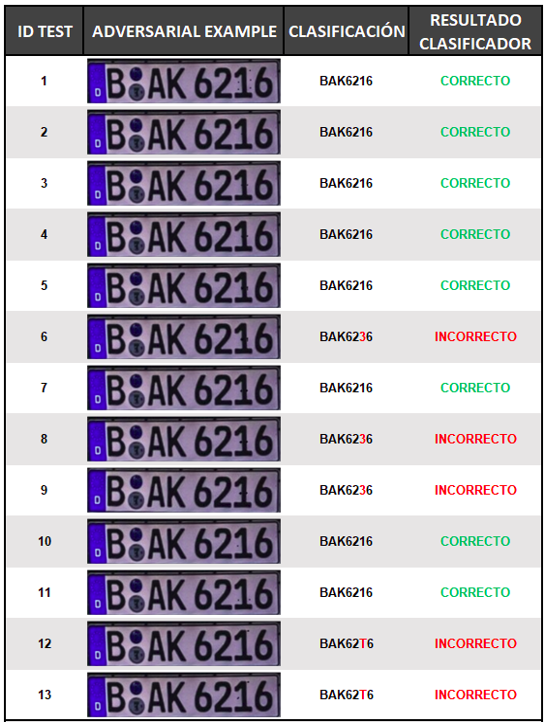
\includegraphics[scale = 0.85]{Figures/figura_68_1.PNG}
    \label{fig:68_1}
\end{figure}

\begin{figure}[!h]
    \centering
    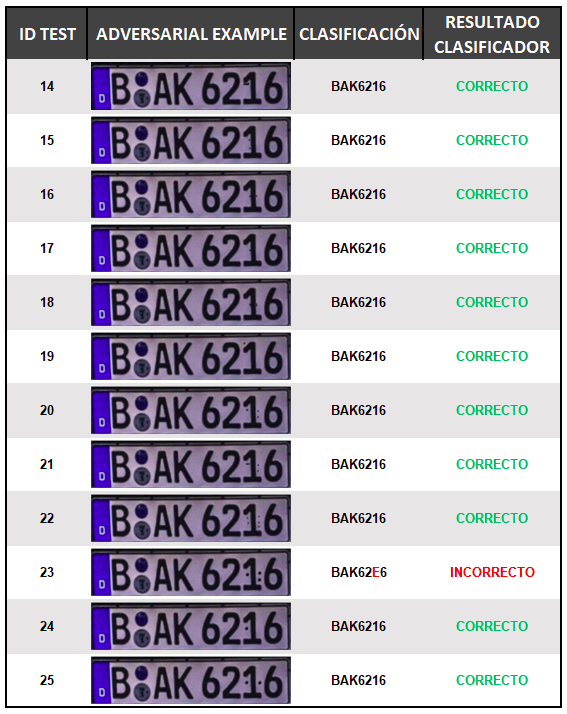
\includegraphics[scale = 0.85]{Figures/figura_68_2.PNG}
    \decoRule
    \caption[Ejemplos adversarios creados por fuerza bruta. placa matrícula alemana.
]{Ejemplos adversarios creados por fuerza bruta. placa matrícula alemana.}
    \label{fig:68_2}
\end{figure}


\section{Placa matrícula española}
Ejemplos adversarios físicos de ataque de fuerza bruta para confundir la interpretación del dígito 1 en modelo Wpod-Net [60] con placa matrícula española.

\begin{figure}[!h]
    \centering
    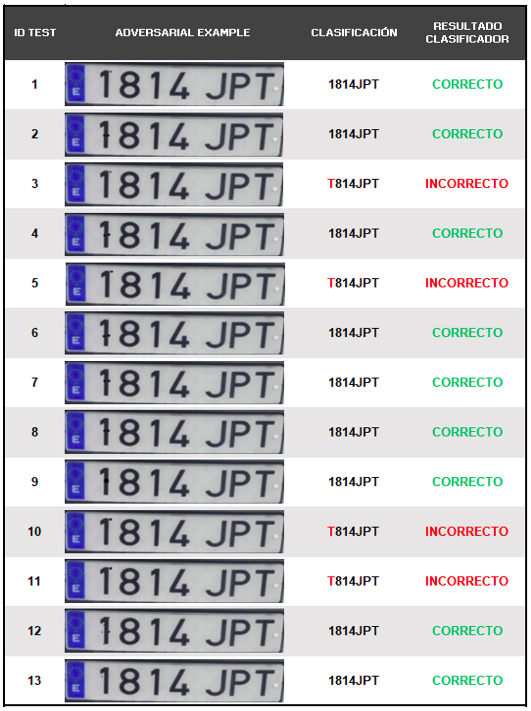
\includegraphics[scale = 0.85]{Figures/figura_69_1.PNG}
    \label{fig:69_1}
\end{figure}

\begin{figure}[!h]
    \centering
    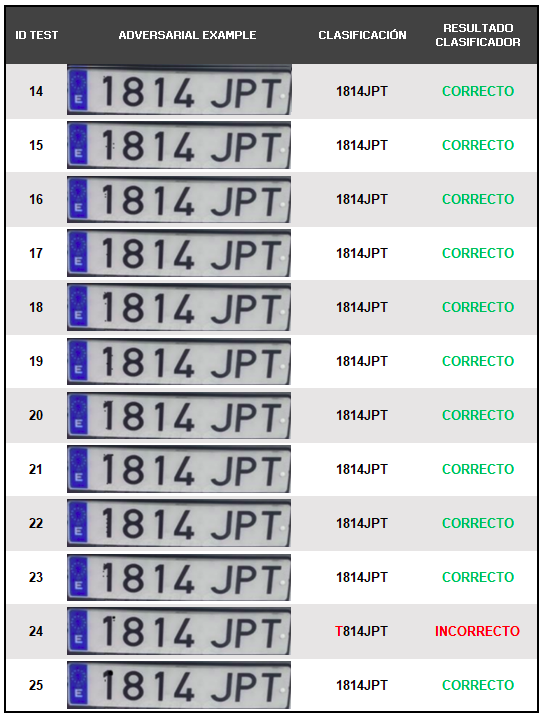
\includegraphics[scale = 0.85]{Figures/figura_69_2.PNG}
    \decoRule
    \caption[Ejemplos adversarios creados por fuerza bruta. placa matrícula española.]{Ejemplos adversarios creados por fuerza bruta. placa matrícula española.}
    \label{fig:69_2}
\end{figure}